\documentclass{article}

\renewcommand{\familydefault}{\sfdefault}  %serifenlose Schrift
\usepackage{helvet} % Schrift: Helvetica


\usepackage{graphicx,graphics,tikz}
\usepackage{amsmath}
\usepackage{amsthm}
\usepackage{amsfonts}
\usepackage{amssymb}
\usepackage{marvosym} % to be able to show male and female symbols with: \Female and \Male
\usepackage{gensymb}
\usepackage[graphics,tightpage,active]{preview}
\PreviewEnvironment{tikzpicture}
\newlength\imagewidth
\newlength\imagescale

\begin{document}

%\pgfmathsetlength{\imagewidth}{10cm} % desired displayed width of image
%\pgfmathsetlength{\imagescale}{\imagewidth/2000} % pixel width of image
% adjust scale of tikzpicture (and direction of y) such that pixel
% coordinates can be used for drawing overlays:
\usetikzlibrary{backgrounds}

\begin{tikzpicture}%[x=\imagescale,y=-\imagescale]

\scalebox{0.9}{
\node at (0,1.5) {\textit{Fucus serratus}};
\node at (0,0) {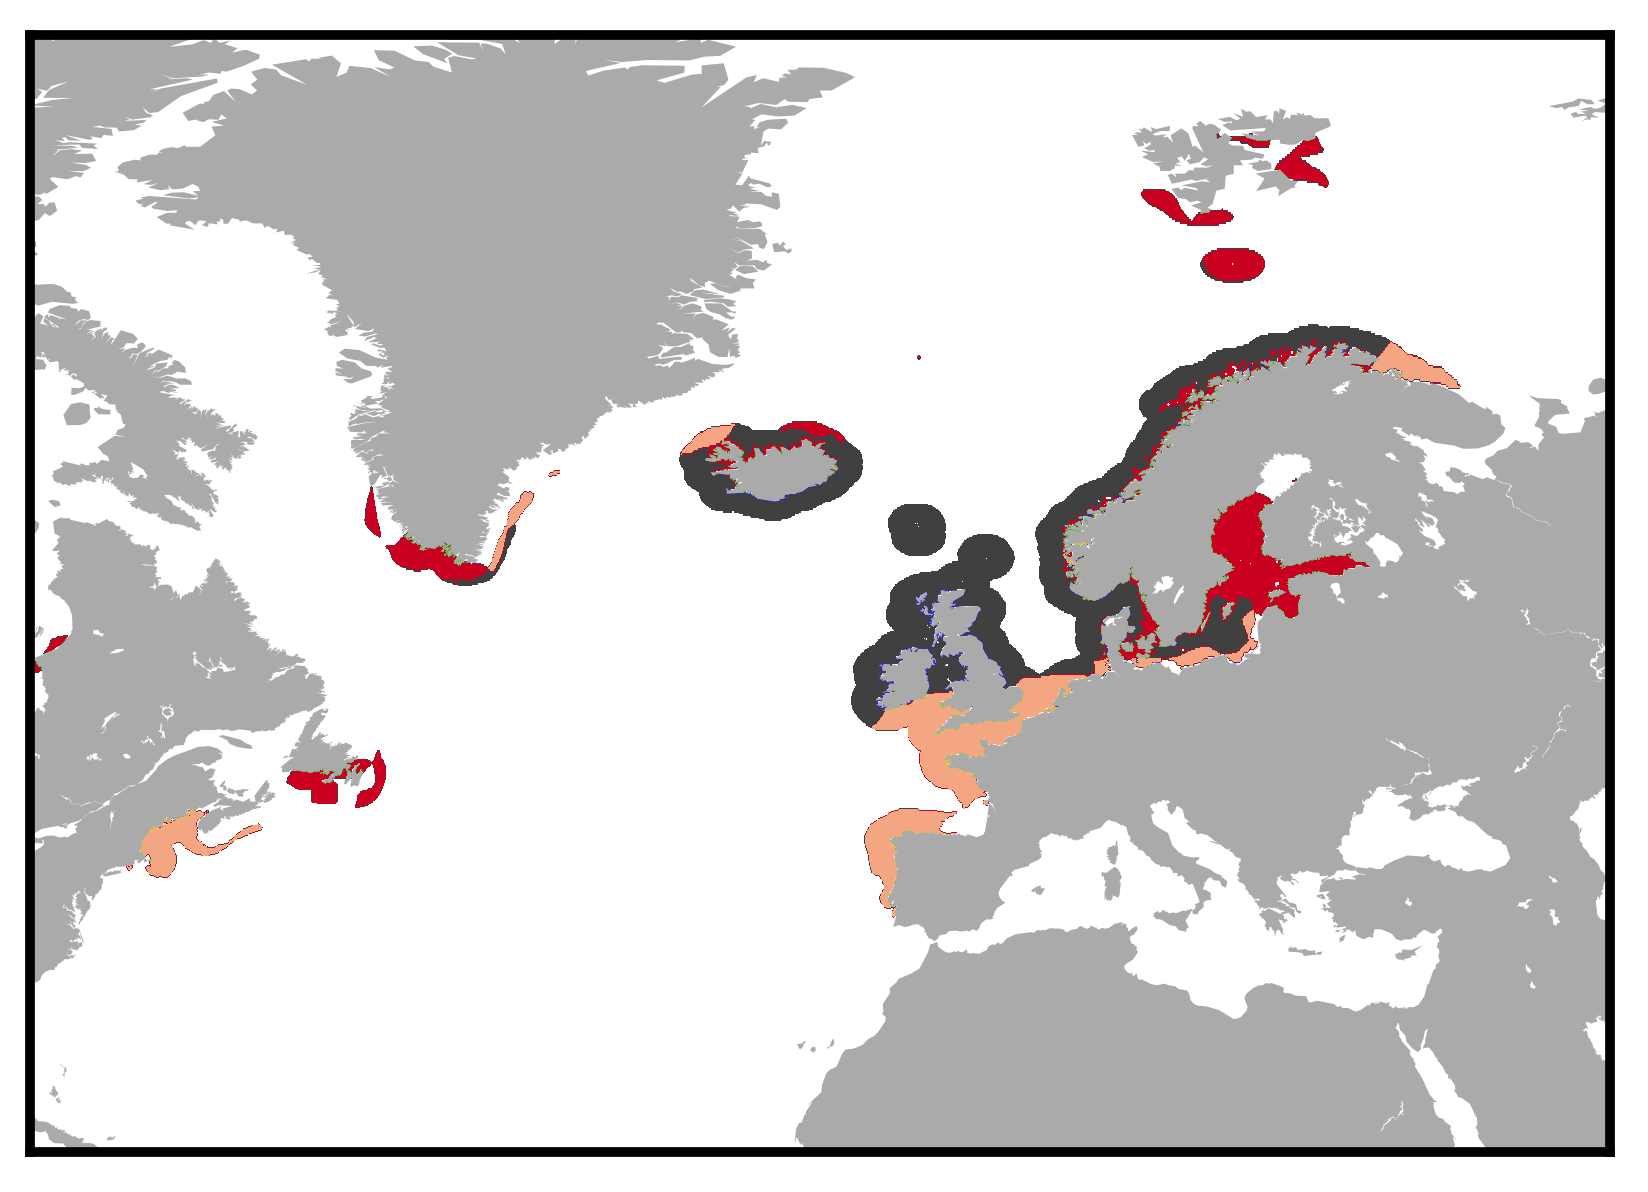
\includegraphics[width=3.3cm]{Fs2200.png}};
\node at (4,1.5) {\textit{Fucus vesiculosus}};
\node at (4,0) {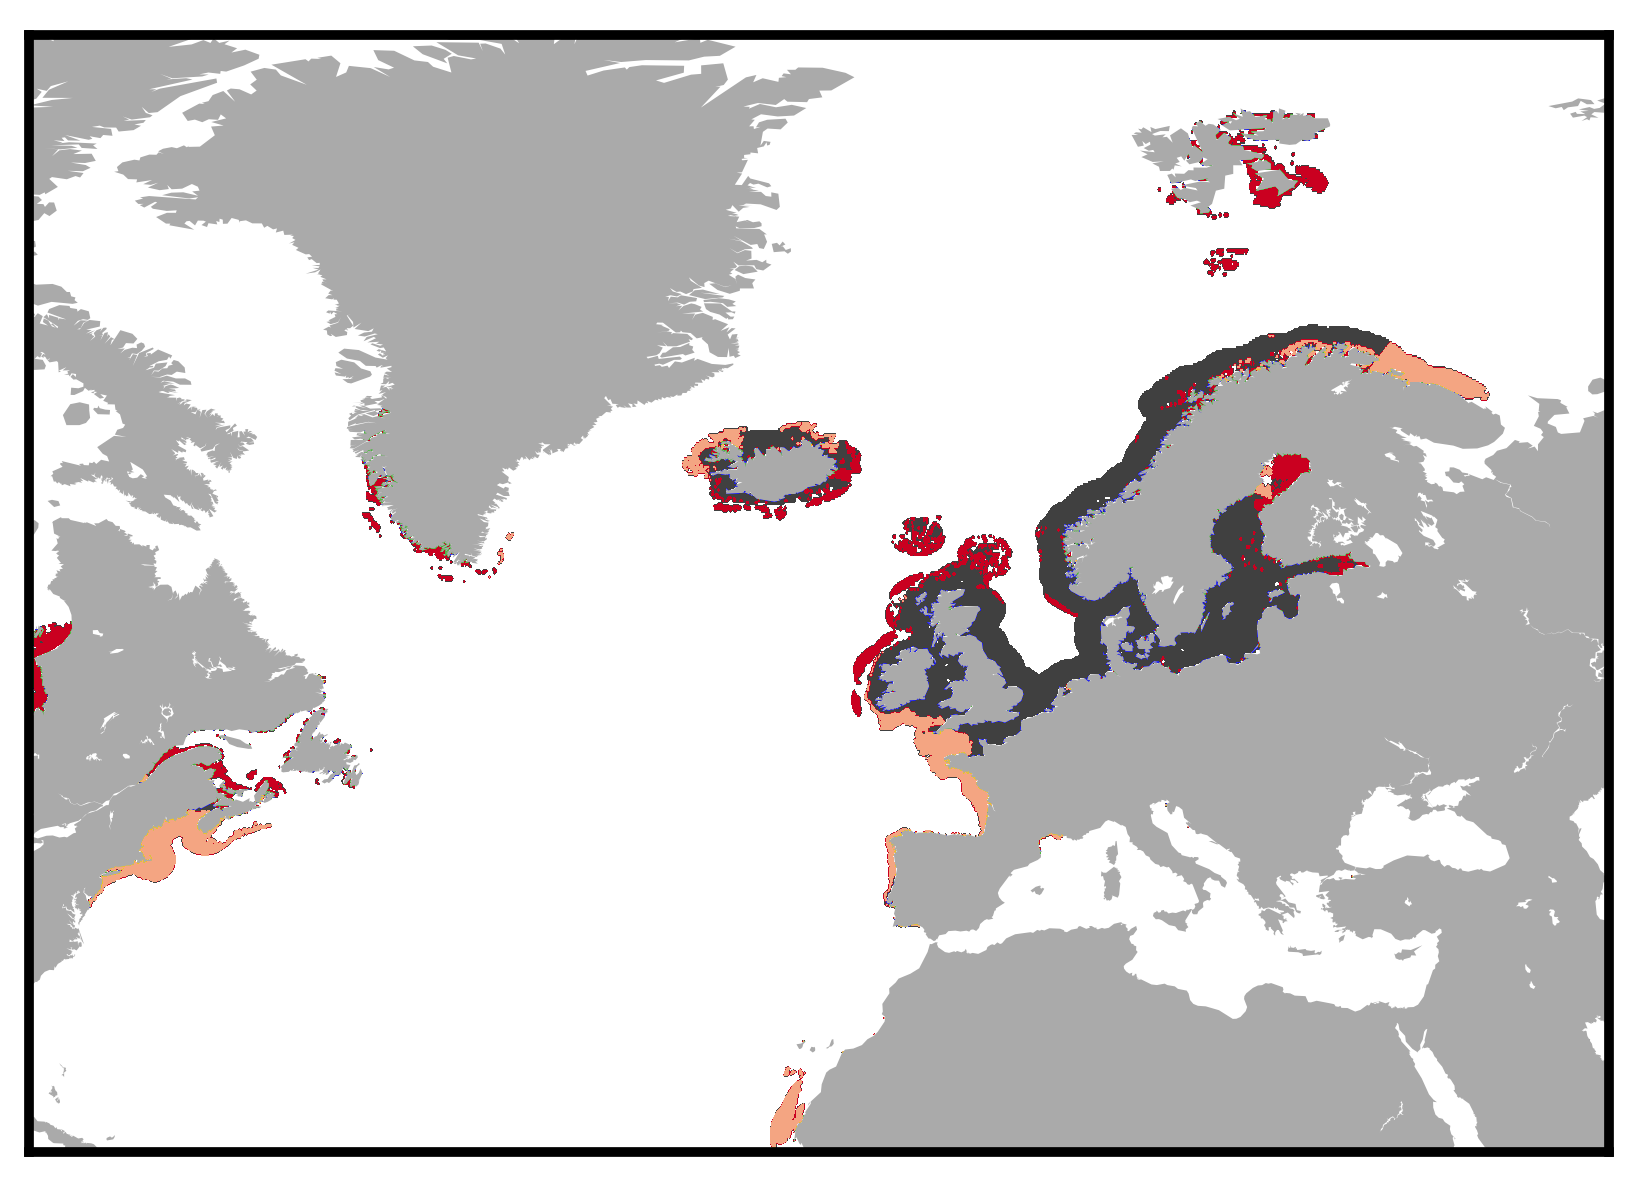
\includegraphics[width=3.3cm]{Fv2200.png}};
\node at (8,1.5) {\textit{Ascophyllum nodosum}};
\node at (8,0) {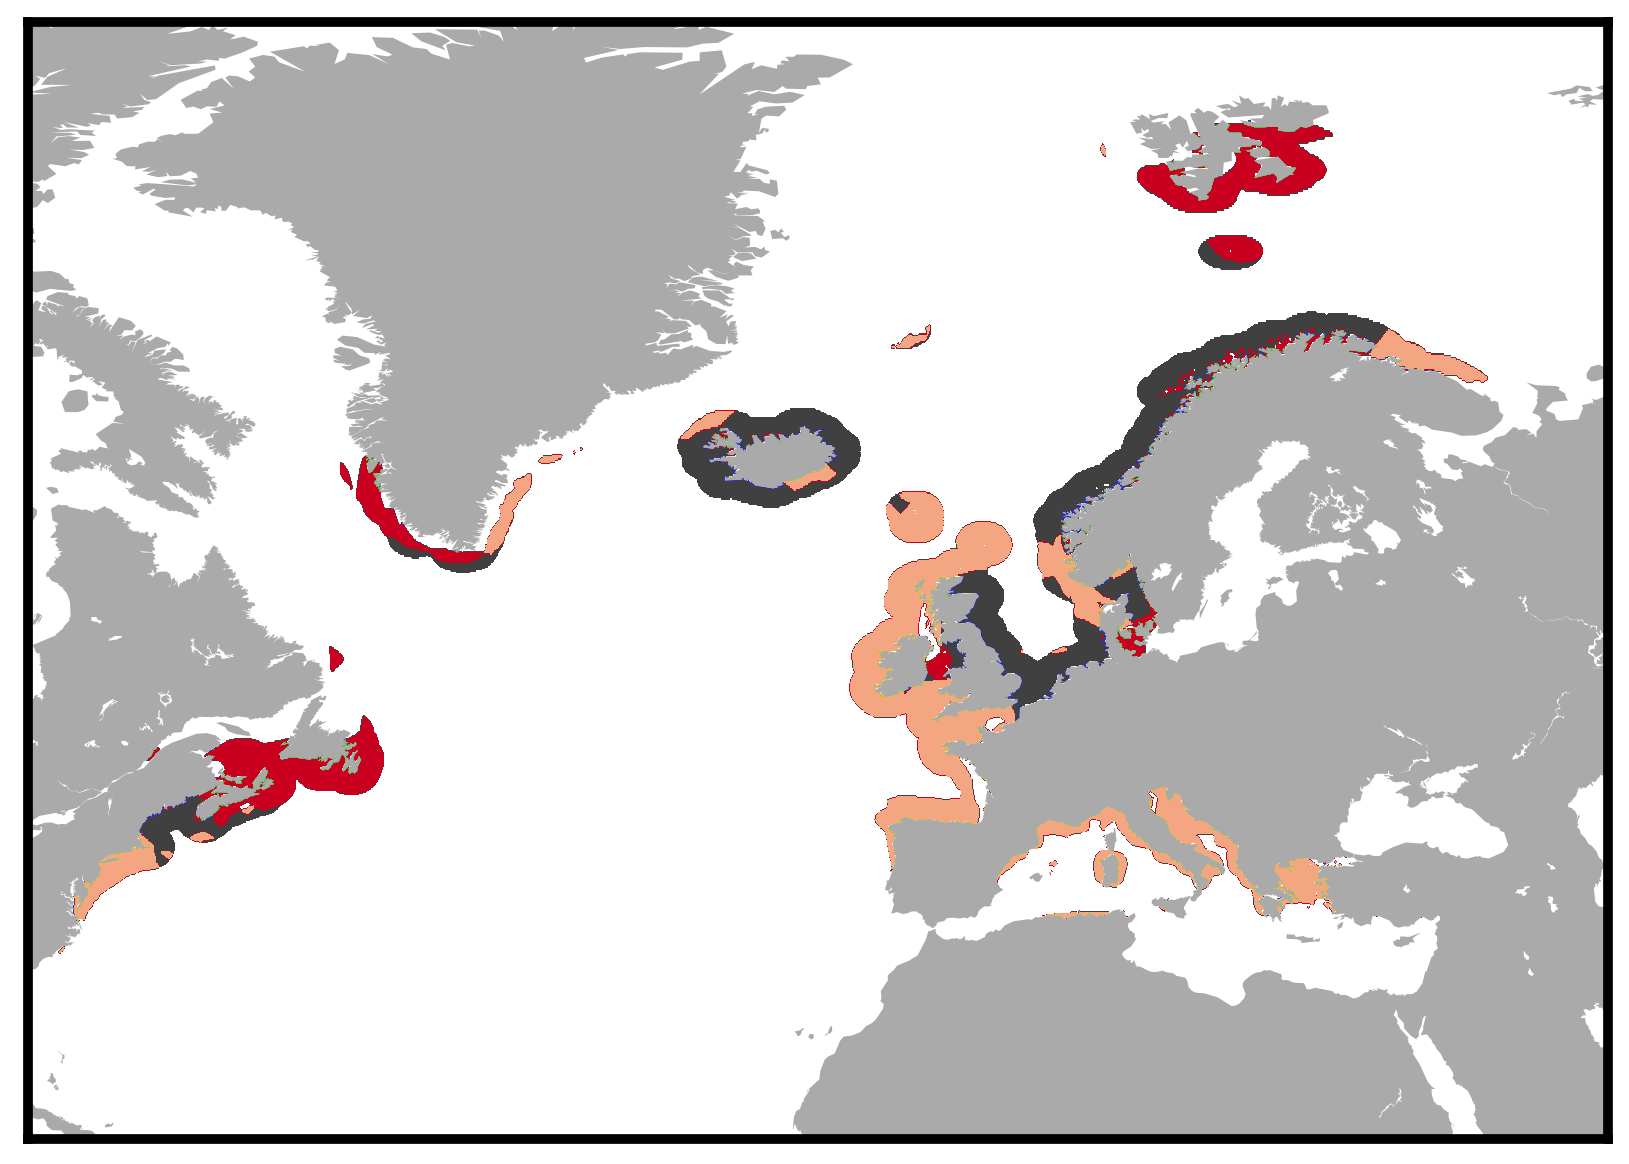
\includegraphics[width=3.3cm]{An2200.png}};

\node at (0,-1.5) {\textit{Fucus distichus}};
\node at (0,-3.5) {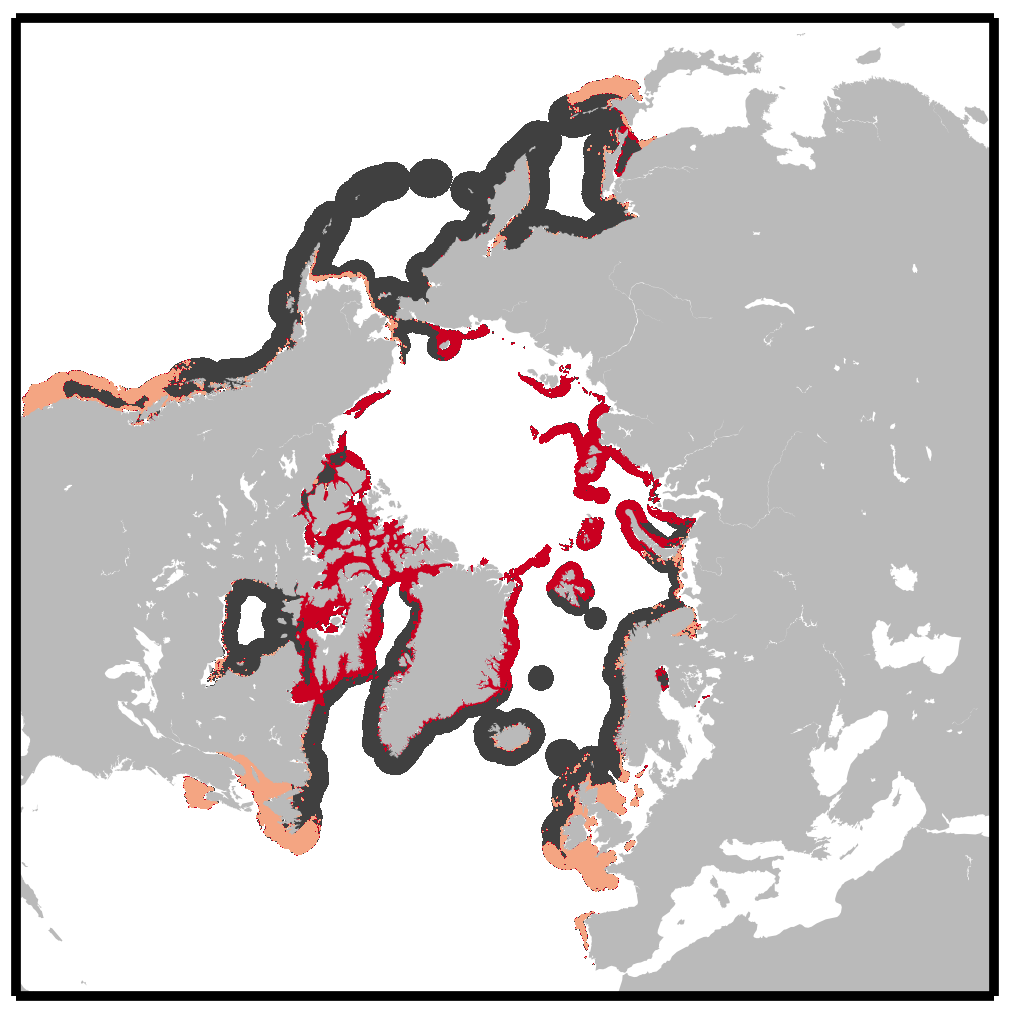
\includegraphics[width=3.3cm]{Fd2200.png}};

\node at (5,-2) {
\includegraphics[width=5cm]{ENMLegend.png}};

%\node <2>[anchor=west,color=green!80!black, text width=6cm, text centered] at (-2.5,0.2) {\small{Habitat gain in the Arctic}};
%\node <3>[anchor=west,color=yellow!80!black, text width=6cm, text centered] at (-2.5,0.2) {\small{Habitat loss in warm temperate areas}};
}


\end{tikzpicture}

\end{document}